\section{Myographie}

% Vergleich mit Röntgenaufnahme: 1. Myonen statt Röntgen-> höhere Reichweite
% Die Myographie ist eines in den Letzten Jahren immer mehr an Fahrt gewinnendes 
% Forschungsfeld. Da sie mit kosmischen Myonen funktioniert, erlaubt
% es ihr eine um Größenordnungen höhere Reichweite als z.B. die Röntgentomographie.

Die Myographie ist wie die Röntgentomografie, ein bildgebendes Verfahren.
Sie verwendet statt künstlich erzeugter Röntgenstrahlung bereits natürlich vorhandene kosmische Myonen.
Da Myonen einen wesentlich geringeren Wirkungsquerschnitt als Röntgen-Photonen
haben und teils sehr hohe Energien besitzen, haben sie eine wesentlich höhere Reichweite
als Röntgen-Photonen. Das ermöglicht der Myographie je nach 
angepeilter Präzision, Größe des Detektors und vorhandener Messzeit
eine Reichweite von mehreren Kilometern und ist daher
für weitläufige Untersuchungen größerer Strukturen oder des Erdreichs geeignet.
Es wurde z.B. zur Entdeckung noch unbekannter Kammern in der Cheops-Pyramide
verwendet\cite{pyramiden} oder zur Untersuchung des inneren eines Vulkans\cite{TANAKA2007104}.

% 1. Energieverlust und -ablenkung
Der Energieverlust und die Ablenkung der Myonen hängt von dem Bodenmaterial 
ab, durch das es propagiert.
Die Stärke des Energieverlusts ist proportional zur Dichte des 
Mediums für Energiebereiche der Myographie\footnote{Unter Vernachlässigung des LPM-Effektes bei hohen Energien.}.
Die Stärke der Ablenkung ist bei der Coulomb-Streuung zusätzlich zur 
Kernladungszahl $Z$ des Mediums proportional.
Im Rahmen der Energiebereiche und Distanzen der Myographie
liegt die mittlere Ablenkung bei $\sim \SI{1,5}{°}$ \cite{Alexandrov2017}.

% \marktodo{welche WW sind wie stark und wichtig? Plot aus dem Alexandrov!} 

% 2. Messzeit kann sehr lange werden
Da die Menge der atmosphärischen Myonen mit der Tiefe abnimmt, 
steigt benötigte Messzeit für präzise Messungen.
Die Messzeit lässt sich allerdings verkürzen durch Vergrößerung 
des Detektor Volumens

% 3. unterschied Detektor -> Winkel Auflösung ja/nein kein Bild standardmäßig
Genauso wie die Röntgentomografie einen Röntgenschirm braucht, der die Röntgenstrahlen 
"detektiert", verwendet die Myographie einen Teilchendetekor für Myonen.
Die einfachste Form eines Detektors für die Myographie zählt die Anzahl der Myonen die 
den Detektor pro Zeiteinheit durchqueren.
%  \marktodo{Vielleicht kurz erwähnen was für Arten von Detektoren möglich sind bzw. wie so eine detektion funktionieren kann.}
In Kombination mit der Messzeit lässt sich 
dann eine Rate angeben, wie viele Myonen pro Zeiteinheit durch den Detektor detektiert werden.

% Eine Vergrößerung ist allerdings nicht immer möglich aufgrund der Größe des Messraums
% und erhöht die Kosten des Projekts.

% Zusätzlich nimmt mit längeren Wegstrecken die Streuung der Myonen an den Atomen zu.
% Wenn der Detektor die Richtung der Myonen messen soll, wird diese also mit steigender Tiefe
% immer unschärfer.

% Die gemessene Rate $\frac{N_\mathrm{Myon}}{\mathrm{cm}^2 \; \mathrm{min}}$ 
% liefert erst eine Aussage, wenn\dots
% \marktodo{
%     ist die Reihenfolge des Erklärens sinnvoll? Sind das die wesentlichen Punkte um in die Myographie einzuleiten? \\\\
%     \marktodo{kleine ($\SI[]{\approx  1}[]{m^3}$) bis große ($\SI[]{< 1}[]{km^3}$) Strukturen untersuchbar.} 
%     \\
%     von JM:
%     Auch wenn es vermutlich in den nächsten Unterkapiteln noch ausführlicher erläutert wird, 
%     fehlt mir hier ein wenig der Grundgedanke, wie man denn jetzt genau Myographie verwenden 
%     kann. Du schreibst zwar explizit dass es "wie bei der Röntgenuntersuchung ist", 
% \\
%     aber vielleicht solltest du trotzdem erwähnen dass
%          mehr Masse pro Strecke = weniger Myonen ist,
%     und vielleicht auch erwähnen dass man 
%         mit einer Richtungsabhängigen Messung dann auch Profile erstellen kann.
% }

\textbf{Detektion eines Untergrundschachts mithilfe der Myographie} \\
%  \marktodo{anwendungsbeispiel vs experiment} 
Zur Veranschaulichung der Myographie wird im Folgenden ein Beispiel im Detail erklärt.
In \cite{Alexandrov2017} wird das  FIAN-SINP MSU Experiment beschrieben.
Ein Photo-Emulsions-Detektor hat über eine Messzeit von 4 Monaten   
Myonen richtungsabhängig gezählt.
Dieser wurde in einem Raum $\SI[]{30}[]{m}$ unterhalb der Erdoberfläche 
installiert. 
Der Versuchsaufbau ist in Abb. \ref{fig:alexandrov_messaufbau} zu sehen.

Ziel des Versuchs war es herauszufinden, ob der Aufzugsschacht in der Messung sichtbar ist. 
Parallel wurde eine Simulation der Messung zum Vergleich erstellt.
In Abb. \ref{fig:alexandrov_ergebnisse} sind die Ergebnisse zu sehen.
Der rote Kasten zeigt die Richtung des Aufzugsschachts.
Der rote Bereich innerhalb des Kastens bedeutet eine hohe Intensität an Myonen aus dieser Richtung.
Da in dem Schacht lediglich Luft ist, verlieren die Myonen beim Propagieren
durch die Luft wesentlich weniger Energie als im Erdreich, daher wurden aus dieser Richtung besonders viele Myonen detektiert.

Zusammenfassend konnte also erfolgreich mithilfe eines Photo-Emulsions-Detektors
 ein Untergrundschacht entdeckt bzw. gemessen werden.

\begin{figure}
    \centering
    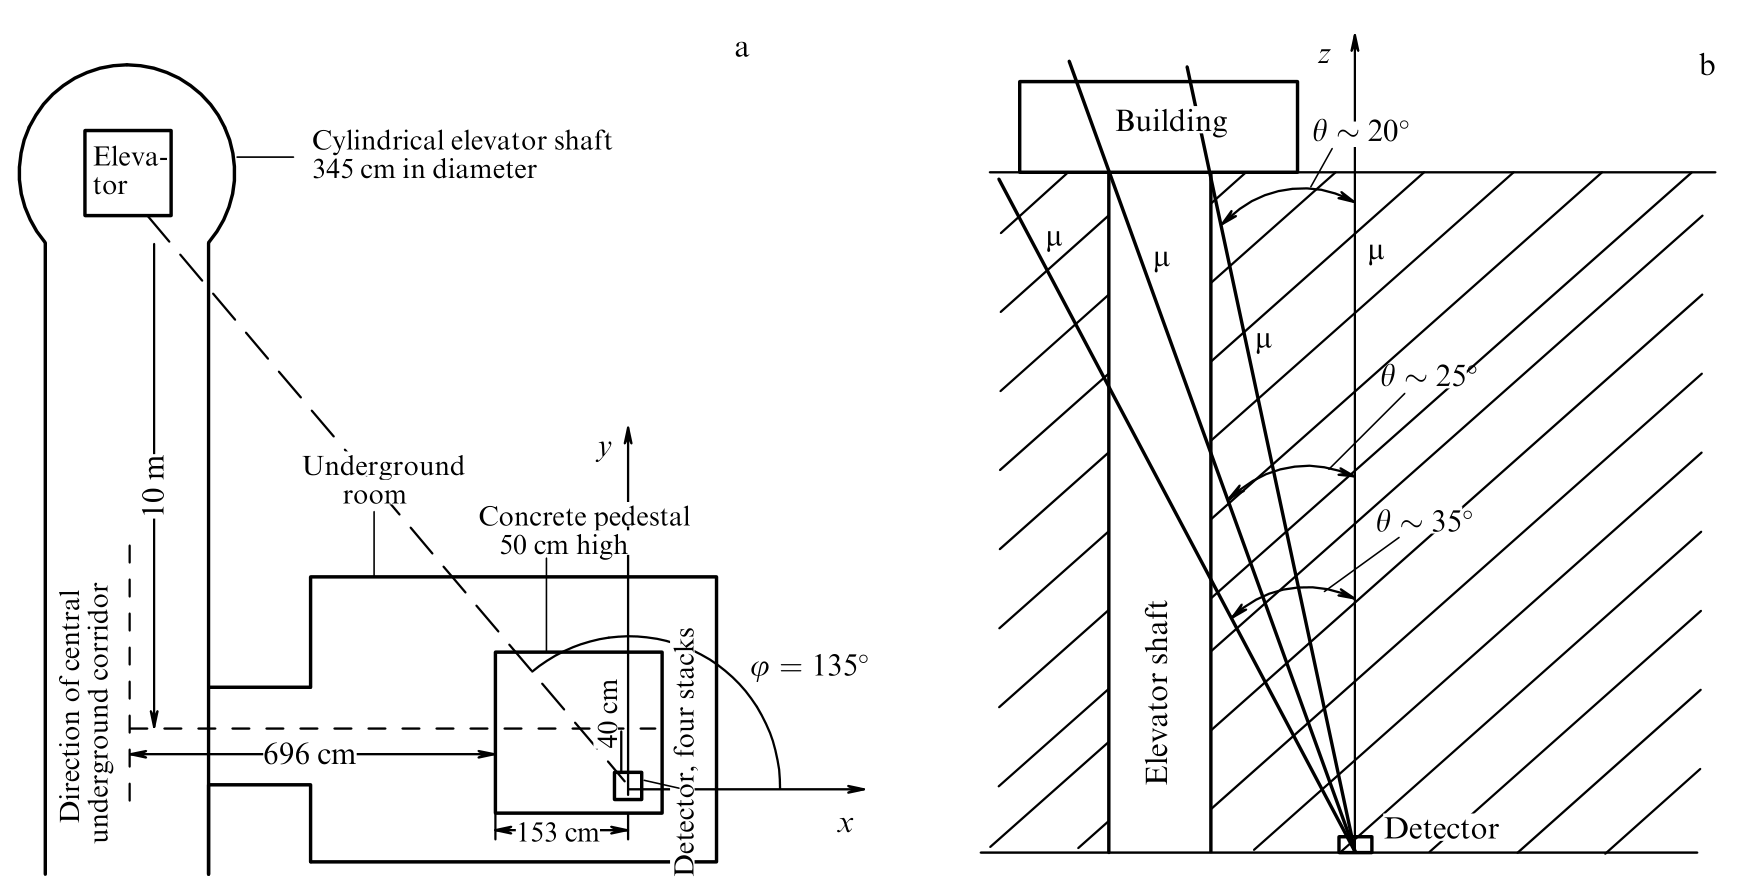
\includegraphics[width=0.9\textwidth]{alexandrov_messaufbau}
    \caption{Horizontale (a) and vertikale (b) Sicht auf das FIAN-SINP MSU Experiment \cite{Alexandrov2017}.
    Der Detektor hat in einer Tiefe von \SI[]{30}[]{m} über einen Zeitraum von 4 Monaten
    Myonen richtungsabhängig gemessen. Ziel war es, den Aufzugsschacht auflösen zu können.
    Die Anordnung der Koordinatenachsen ist im Detektorsystem angegeben.}
    \label{fig:alexandrov_messaufbau}
\end{figure}

\begin{figure}
    \centering
    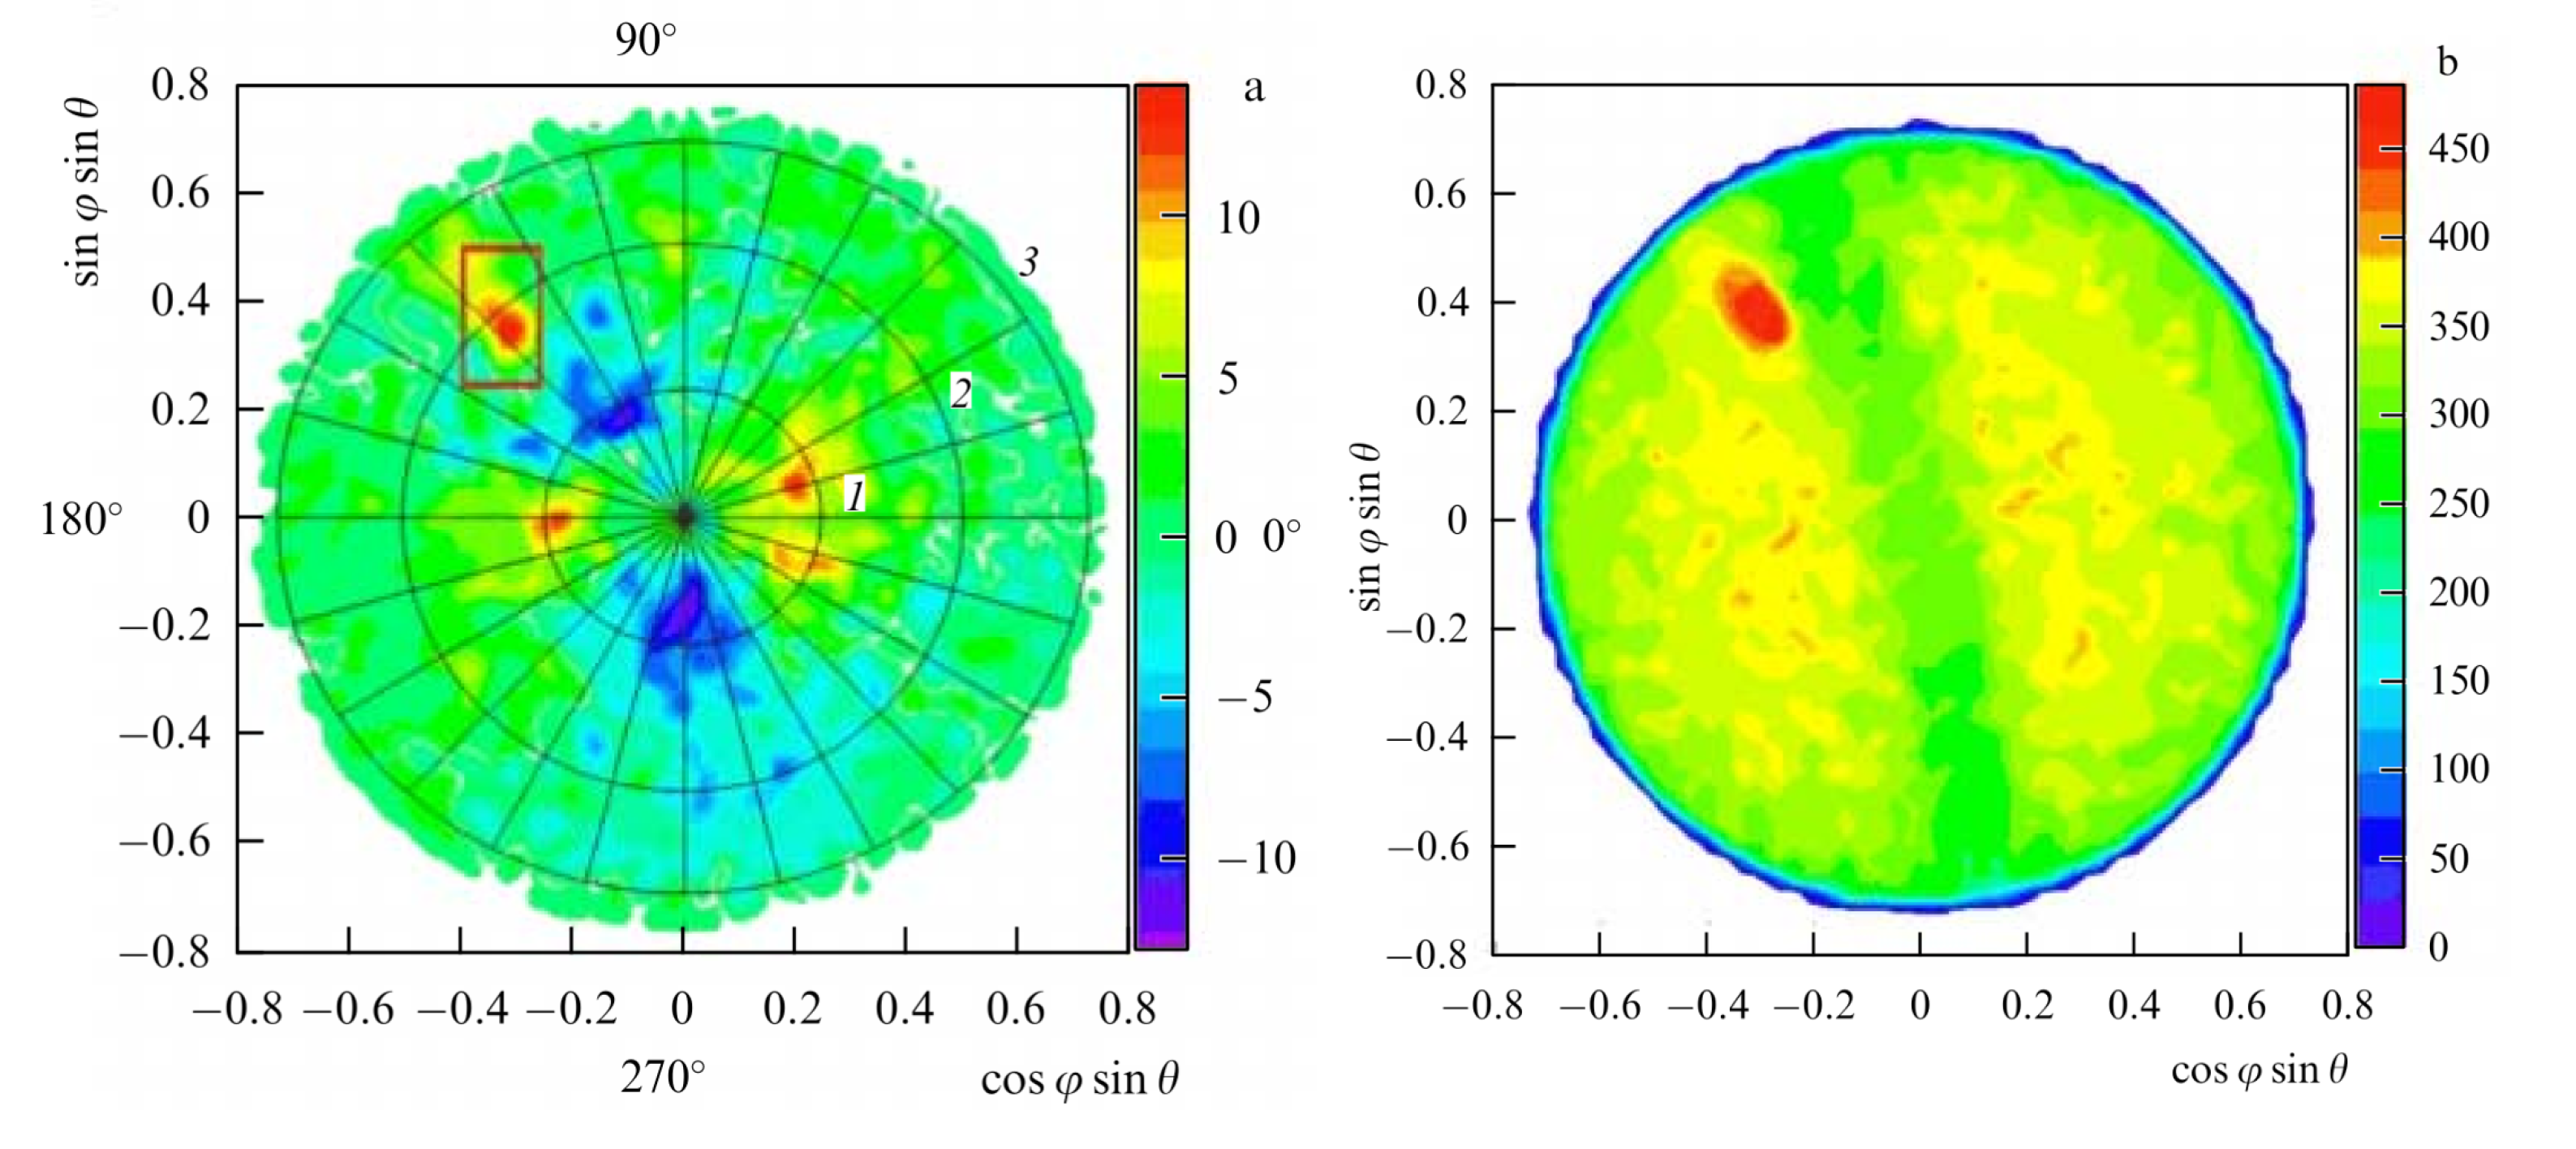
\includegraphics[width=0.93\textwidth]{alexandrov_beide}
    \caption{
        (a) Zweidimensionale Spurendichteverteilung der Myonen
        \SI[]{30}[]{m} unter der Erde. 
        Das rote Rechteck markiert den Blickwinkel in Richtung des Aufzugschachts. 
        Die Kreise nummeriert mit 1, 2 und 3, markieren jeweils die Zenitwinkel $\theta = 15°$, $30°$ und $45°$
        %
        (b) 
        Simulierte Verteilung aus der Simulation. Der deutlich zu erkennende rote Fleck
        repräsentiert einen hohen Myonenfluss aus der Richtung des Aufzugsschachts.
        Die Verteilungen der Spurendichte sind in Form der Variablen $\sin \phi \sin \theta$ 
        und $\cos \phi \sin \theta$ dargestellt. Sie repräsentieren den Einfallswinkel der detektierten Myonen
        gegenüber der Senkrechten zur Detektorebene.
        \cite{Alexandrov2017}
    }
    \label{fig:alexandrov_ergebnisse}
\end{figure}

% - $\frac{I_{det}}{I_0} \sim \sum m$
%   Myonen Abschwächung gegenüber Oberfläche ist proportional zur Masse des 
% durchquerten Materials


% - Detektoren messen Myonen-Intensität (N, E, $\phi$)
%     - Erkenntnisse über Beschaffenheit des Masse “über” einem
% - anhand eines Beispiels:
% - Man ist in einer erforschten Pyramide und möchte herausfinden ob es noch unentdeckte Hohlräume gibt.
% - $\rho * V = m$
%     - Myographie liefer die die Masse quasi, denn je mehr masse durchquert wird desto mehr Energie verlieren die Myonen und zerfallen
%     - man gibt der Myographie noch V und bekommt so rho des materials → Eigenschaften des gemessens Materials
% - Einordung der myographie
%     - strahlungsquelle und intensität immer vorhanden und bekannt
% - Detekoren auch ohne Strom betreibbar
% - viele Anwendungsfelder
% - unterscheidung zwischen myographie und myon tomographie